\documentclass[12pt,conference]{IEEEtran}
\hyphenation{op-tical net-works semi-conduc-tor}
\usepackage[pdftex]{graphicx}
\usepackage{textcomp}
\usepackage{hyperref}
\usepackage{cite}
\usepackage{listings}
\lstset{
	basicstyle=\ttfamily,
	showstringspaces=false,
	escapechar=\%,
	breaklines=true,
	numbers=left,
	xleftmargin=2em
}

\begin{document}

\title{Time Randomization to Thwart Concurrency Bug Exploitation}
\author{\IEEEauthorblockN{David M. Tagatac}
\IEEEauthorblockA{Department of Computer Science\\
Columbia University, New York, NY 10027\\
Email: dtagatac@cs.columbia.edu}}
\maketitle

\section{Introduction}
With the pervasiveness of multicore architectures, multithreading is an important - and often necessary - tool when programming for performance.  However, programming with multiple threads is generally more difficult than programming for serial execution.  Each thread has the potential to contain any bug of a serial program, and on top of that, the uncertain interleaving of concurrent threads has the potential for concurrency bugs (e.g. data races).

Lu et al. did a survey of concurrency bugs \cite{Lu2008}, and Yang et al. has demonstrated that attacks on buggy multithreaded programs are a real concern \cite{Yang2011}.  Much of the effort in combating this threat has gone into tools and systems which detect data races in order to aid debugging \cite{Savage1997, Flanagan2004, Laadan2011, Pratikakis2011, Kasikci2013}.  An alternative approach is to guide multithreaded programs into memoized synchronization schedules \cite{Cui2011}.  This approach does not dwell on race detection, but rather on removing the nondeterminism from the portions of multithreaded programs where races are most likely.  However, schedule memoization in its most automated form is still susceptible to attack whenever the attacker can trigger a different schedule by changing the input.

We address the threat of concurrency attacks from yet another angle.  Much like the way that address space layout randomization thwarts attacks that depend on absolute and/or relative code and data addresses in memory, we propose to thwart concurrency attacks that depend on specific thread timing by randomizing the delays between and among threads.  Like the memoization approach described above, we also focus on the synchronization schedule (the interleaving of the various threads in a multithreaded program).  However, instead of removing nondeterminism to increase reproducibility, we attempt to randomize the synchronization schedule to remove the possibility that the relative timing of two (or more) threads can be studied and used to craft an attack.  For this subset of concurrency attacks which depend on thread timing, we hypothesize that random injection of timing delays between concurrent threads will reduce the chance of any specific attack's success.  If such an attack can address different thread timing with correspondingly different input timing, at least randomization increases the cost to the attacker to determine the appropriate input timing; moreover, that knowledge is only useful for one system until the next randomization. 

\section{Preliminary Results}
\begin{figure}
\begin{lstlisting}[firstnumber=43]
static inline long do_mmap2(
unsigned long addr, unsigned long len,
unsigned long prot, unsigned long flags,
unsigned long fd, unsigned long pgoff)
{
	int error = -EBADF;
	struct file * file = NULL;

	flags &= ~(MAP_EXECUTABLE | MAP_DENYWRITE);
	if (!(flags & MAP_ANONYMOUS)) {
		file = fget(fd);
		if (!file)
			goto out;
	}
	%\textbf{udelay(100);}%
	down_write(&current->mm->mmap_sem);
	error = do_mmap_pgoff(file, addr, len, prot, flags, pgoff);
	up_write(&current->mm->mmap_sem);

	if (file)
		fput(file);
out:
	return error;
}
\end{lstlisting}
\caption{An example targeted timing delay in the CentOS Linux kernel 2.4.21 in function do\_mmap2 in arch/i386/kernel/sys\_i386.c, line 57.}
\label{fig_mmapcode}
\end{figure}
\begin{figure}
\centering
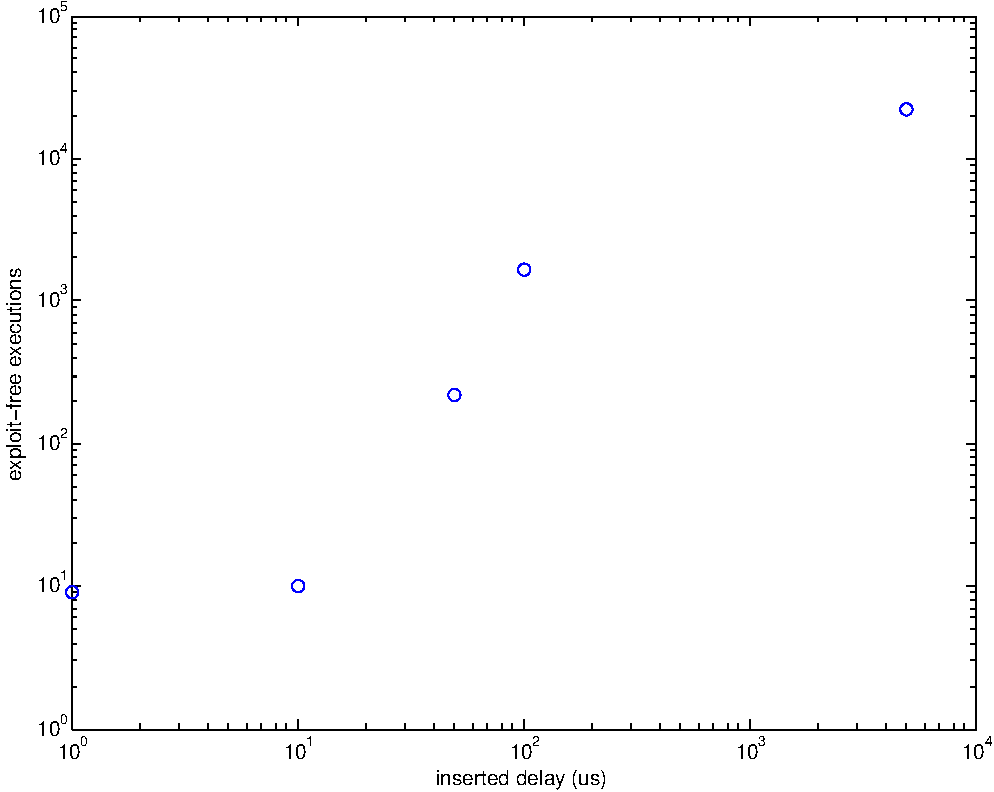
\includegraphics[width=\columnwidth]{prelimgraph}
\caption{The effect of placing targeted timing delays in the (buggy) CentOS Linux kernel 2.4.21.  Delays between 0 and 5,000{\textmu}s were inserted strategically to alter concurrent thread timing, and the number of failed exploit script runs prior to a successful exploit strictly increased with the length of the inserted delay.}
\label{fig_prelimgraph}
\end{figure}
To motivate the plausibility of our approach, we first tested the effects of targeted timing delays in buggy multithreaded code for which we have an exploit script.  The CentOS 3.9 kernel (from Linux 2.4.21) contains a critical concurrency bug that causes a system hang when exploited \cite{CVE2006-4814}.  The bug is a deadlock on the mmap semaphore `mmap\_sem' that is triggered by a specific interleaving of concurrent threads, one calling the mmap system call and the other calling the mincore system call.  The Red Hat bug report \cite{RHELbug180663} provides a script which creates two threads - one that repeatedly calls mincore in a loop, and another that repeatedly calls mmap in a loop.  By placing calls to usleep() just before the call to down\_write on mmap\_sem in the i386 architecture-specific implementation of mmap (Figure \ref{fig_mmapcode}), we were able to alter the timing of the thread interleaving.  We observed that the number of exploit script runs required for a successful exploit strictly increased with the duration of the sleep inserted (Figure \ref{fig_prelimgraph}).

\section{Experiment}
After observing that targeted timing delays reduce the success rate of at least one concurrency bug exploit, the next step is to show that randomized timing delays have a similar effect.  Our approach is to rewrite buggy multithreaded binaries, for which we have exploit scripts in hand, in the following way:
\begin{enumerate}
	\item Replace all function calls with jumps to variable-length NOP loops, different for each function.
	\item At the end of these loops, jump to the originally intended function.
	\item Randomize the NOP loop lengths on each rewrite.
\end{enumerate}
\newpage{}
In this way, we can change the program timing by introducing randomness between experiments.  In a real-world scenario this would correspond to program rewrites at boot time, or some other periodic interval.

If the reduction in exploit success justifies the overhead of the timing delays, thread timing randomization could be an important defense against concurrency attacks.

\bibliographystyle{IEEEtran}
\begin{thebibliography}{10}
\bibitem{Lu2008}
S. Lu, S. Park, E. Seo and Y. Zhou, "Learning from mistakes - A Comprehensive Study on Real World Concurrency Bug Characteristics," in \emph{Proceedings of the 13th international conference on Architectural support for programming languages and operating systems} - ASPLOS XIII, New York, NY, 2008.
\bibitem{Yang2011}
J. Yang, A. Cui, S. Stolfo and S. Sethumadhavan, "Concurrency Attacks," in HotPar'12 \emph{Proceedings of the 4th USENIX conference on Hot Topics in Parallelism}, Berkeley, CA, 2011.
\bibitem{Savage1997}
S. Savage, M. Burrows, G. Nelson, P. Sobalvarro and T. Anderson, "Eraser: a dynamic data race detector for multithreaded programs," \emph{ACM Transactions on Computer Systems}, vol. 15, no. 4, pp. 391-411, 1997.
\bibitem{Flanagan2004}
C. Flanagan and S. N. Freund, "Atomizer: a dynamic atomicity checker for multithreaded programs," in \emph{18th International Parallel and Distributed Processing Symposium}, 2004. Proceedings., 2004.
\bibitem{Laadan2011}
O. Laadan, C.-C. Tsai, N. Viennot, C. Blinn, P. S. Du, J. Yang and J. Nieh, "Finding Concurrency Errors in Sequential Code—OS-level, In-vivo Model Checking of Process Races," in \emph{Proceedings of the 13th USENIX conference on Hot topics in operating systems}, 2011.
\bibitem{Pratikakis2011}
P. Pratikakis, J. S. Foster and M. Hicks, "LOCKSMITH: Practical Static Race Detection for C," \emph{ACM Transactions on Programming Languages and Systems}, vol. 33, no. 1, pp. 1-55, 2011.
\bibitem{Kasikci2013}
B. Kasikci, C. Zamfir and G. Candea, "RaceMob: Crowdsourced Data Race Detection," in \emph{Proceedings of the Twenty-Fourth ACM Symposium on Operating Systems Principles} - SOSP '13, New York, NY, 2013.
\bibitem{Cui2011}
H. Cui, J. Wu, J. Gallagher, H. Guo and J. Yang, "Efficient Deterministic Multithreading through Schedule Relaxation," in \emph{Proceedings of the TwentyThird ACM Symposium on Operating Systems Principles} SOSP 11, 2011.
\bibitem{CVE2006-4814}
CVE-2006-4814. \url{http://www.cvedetails.com/cve/CVE-2006-4814/}
\bibitem{RHELbug180663}
Red Hat Bugzilla --- Bug 180663.\\\url{https://bugzilla.redhat.com/show_bug.cgi?id=180663}
\end{thebibliography}


\end{document}


